\chapter{Proofs and complements of Chapter~\ref{chap:ICALP}}
\minitoc\mtcskip

\section{Proof of Lemma~\ref{lem:compass_hom_gen}}\label{proof:lem:compass_hom_gen}

\begin{lemma*}[\ref{lem:compass_hom_gen}]
Let $\cG=(\bbP_\bbD,\cL)$. $\cG$ is a fulfilling homogeneous compass $\varphi$-structure if and only if, for every pair $x,y \in \mathpzc{S}$,  we have: 
\begin{itemize}
    \item $\cL(x,y-1)\cL(x+1, y)\genDphi \cL(x, y)$ if $x<y$, and 
    \item $\reqD(\cL(x,y))=\emptyset$ if $x=y$.
\end{itemize}
\end{lemma*}

\begin{proof}
$(\Rightarrow)$
Let us consider $x,y \in \mathpzc{S}$.
First we note that, since $\cG$ is fulfilling, it must be $\reqD(\cL(x,y))=\emptyset$ whenever $x=y$.
Otherwise, if $x<y$, we consider the labelings $\cL(x,y-1)$ and $\cL(x+1, y)$. By the homogeneity property
of Definition~\ref{def:hom_compass}, $\cL(x,y)\cap\AP = \cL(x,y-1) \cap \cL(x+1,y)\cap \AP$: the first condition 
of Definition~\ref{def:d_generator} holds. 
% Moreover, by the temporal consistency of $\cG$ (Definition~\ref{def:compassstructure}), $ \cL(x,y)\Dphi 
% \cL(x,y-1)$ and thus for every $\BD \psi \in \cL(x,y)$ we have $\BD\psi,\, \psi \in \cL(x,y-1)$. 
% %
% %
% It easily follows that both  $\reqD(\cL(x,y-1))\subseteq \reqD(\cL(x,y))$ and $\obsD(\cL(x,y-1))\subseteq \reqD(\cL(x,y))$. Analogously we have $\reqD(\cL(x+1,y))\subseteq \reqD(\cL(x,y))$ and $\obsD(\cL(x+1,y))\subseteq \reqD(\cL(x,y))$.
Moreover,
since $\cG$ is fulfilling, for every $\psi \in \reqD(\cL(x,y))$ we have that either $\psi\in \cL(x,y-1)$, or   $\psi\in \cL(x+1,y)$, or $\psi \in \cL(x',y')$
for some $x<x'\leq y'<y$. In the first two cases $\psi \in \obsD(\cL(x,y-1)) \cup \obsD(\cL(x+1,y))$. As for the last case,  by Lemma~\ref{lem:transitive_req}, $\obsD(\cL(x',y'))\subseteq \reqD(\cL(x,y-1))$ and $\obsD(\cL(x',y'))\subseteq \reqD(\cL(x+1,y))$,
hence
$\psi \in \reqD(\cL(x,y-1))$ and  $\psi \in \reqD(\cL(x+1,y))$.
We can conclude that $\reqD(\cL(x,y))\subseteq\obsD(\cL(x,y-1)) \cup \obsD(\cL(x+1,y)) \cup  \reqD(\cL(x,y-1)) \cup \reqD(\cL(x+1,y))$. The converse inclusion ($\supseteq$) follows by Lemma~\ref{lem:transitive_req}, hence the second condition of Definition~\ref{def:d_generator} holds. We conclude that $\cL(x,y-1)\cL(x+1, y)\genDphi \cL(x, y)$.

$(\Leftarrow)$ Let us consider $\cG=(\bbP_\bbD,\cL)$ such that, for every pair $x,y \in \mathpzc{S},\, x\leq y$, we have $\cL(x,y-1)\cL(x+1, y)\genDphi \cL(x, y)$ if $x<y$, and $\reqD(\cL(x,y))=\emptyset$ if $x=y$. We have to prove that $\cG$ is a homogeneous fulfilling compass $\varphi$-structure. 

First, we prove consistency w.r.t.\ the relation $\Dphi$.
Let us show that, for all pairs of 
points $(x,y)$ and $(x',y')$ with $(x',y')\subint(x,y)$,
we have $\cL(x,y)\Dphi\cL(x',y')$. 
The proof is by induction on $\Delta =(x'-x) + (y - y')\geq 1$.
If $\Delta=1$, either $(x',y')=(x+1,y)$
or $(x',y')=(x,y-1)$. Let us consider $(x',y')=(x+1,y)$
(the other case is symmetric). Since 
$\cL(x,y-1)\cL(x+1, y)\genDphi \cL(x, y)$,
we easily get that $\cL(x,y)\Dphi \cL(x+1, y)$.
If $\Delta \geq 2$, 
since $(x',y')\subint(x,y)$, then
$(x',y'+1)\subint(x,y)$
or $(x'-1,y')\subint(x,y)$. We only consider
$(x'-1,y')\subint(x,y)$, being the other case symmetric. By the inductive hypothesis, 
$\cL(x,y)\Dphi \cL(x'-1,y')$.
Since $\cL(x'-1,y'-1)\cL(x', y')\genDphi \cL(x'-1, y')$,
we have $\cL(x'-1, y')\Dphi \cL(x',y')$.
 Let us observe that $\Dphi$ is a transitive relation,
and thus $\cL(x, y)\Dphi \cL(x',y')$.

We now show that $\cG$ is fulfilling.
We prove that for every point 
$(x,y)\in\bbP_\bbD$ and for every 
$\psi\in \reqD(\cL(x,y))$, there exists $(x',y')\in\bbP_\bbD,\,(x',y')\subint(x,y)$ such that
$\psi\in\cL(x',y')$. The proof is by induction on 
$y-x\geq 0$. If $x=y$, we have $\reqD(\cL(x,y))=\emptyset$, hence the thesis holds vacuously. 
If $y-x\geq 1$, since 
$\cL(x,y-1)\cL(x+1, y)\genDphi \cL(x, y)$,
we have $\reqD(\cL(x, y))= \reqD(\cL(x,y-1))\cup\reqD(\cL(x+1, y))\cup \obsD(\cL(x,y-1))\cup\obsD(\cL(x+1, y))$. If $\psi \in \obsD(\cL(x,y-1))\cup\obsD(\cL(x+1, y))$, the thesis is verified. If $\psi \in \reqD(\cL(x+1, y))$ (the case $\psi \in \reqD(\cL(x, y-1))$ is symmetric and thus omitted), by the inductive hypothesis, 
$\psi \in \cL(x'',y'')$ for some
$(x'',y'') \subint (x+1, y) \subint (x,y)$. 

It remains to prove that $\cG$ 
is homogeneous. 
We have to show that, for every $(x,y)\in\bbP_\bbD$ and every $p\in \AP$, $p\in \cL(x,y)$
if and only if for every point $(x',x')$, with $x\leq x' \leq y$, we have $p\in \cL(x',x')$.
The proof is by induction on the length of the interval $(x,y)$. If $x=y$
the property trivially holds. Let us consider now $y-x>0$ (inductive step).
By the inductive hypothesis, since $(x+1, y)$ and $(x,y-1)$ are shorter than $(x,y)$, 
we have $p\in \cL(x+1,y)$  (resp., $p\in \cL(x, y-1)$)
if and only if, for every $(x',x')$ with $x+1 \leq x' \leq y$, (resp., $x\leq x'\leq y-1$), $p\in \cL(x',x')$.
Thus $p \in \cL(x+1,y) \cap \cL(x, y-1)$ if and only if
for every $(x',x')$ with $x\leq x'\leq y$, $p\in \cL(x',x')$.
Since $\cL(x+1,y)\cL(x,y-1)\genDphi \cL(x, y)$, we have
$\cL(x, y)\cap \AP = \cL(x+1,y) \cap \cL(x, y-1) \cap \AP$.
Therefore $p\in \cL(x,y)$ if and only if for every $(x',x')$, with $x\leq x'\leq y$, we have $p\in \cL(x',x')$.
 \end{proof}
 
 
\section{Proof of Lemma~\ref{lem:compas_implies_row}}\label{proof:lem:compas_implies_row}

\begin{lemma*}[\ref{lem:compas_implies_row}]
Let $\cG= (\bbP_\bbD,\cL)$ be a fulfilling homogeneous compass $\varphi$-structure. For every $y\in \mathpzc{S}$, $\row_y$ is a $\varphi$-row.
\end{lemma*}

\begin{proof}
Let  $\row_y=\cL(y,y)^{m_0}\cL(y- m_0, y )^{m_1}\cdots\cL(y - \sum_{0\leq i< n} m_i, y)^{m_n}$ 
where, for every $0\leq j\leq n$, $\cL(y - \sum_{0\leq i< j} m_j, y)^{m_j}$ is a maximal substring of identical atoms (note that any $\row_y$ can be represented w.l.o.g.\  in this way, for $m_i> 0$). 
Since $(y,y) \subint  \ldots \subint (0,y)$, by Lemma~\ref{lem:transitive_req}, $\reqD(\cL(y,y))\subseteq \reqD( \cL(y- m_0, y ))\subseteq\ldots \subseteq \reqD(\cL(y - \sum_{0\leq i< n} m_i, y))$.
Moreover, by homogeneity, $(\cL(y,y)\cap \AP) \supseteq (\cL(y- m_0, y )\cap \AP)\supseteq \ldots \supseteq(\cL(y - \sum_{0\leq i< n} m_i, y)\cap \AP )$. 
By maximality, $\cL(y - \sum_{0\leq i< j} m_i, y)\neq \cL(y - \sum_{0\leq i< j-1} m_i, y)$ for every $0<j\leq n$, and thus, since $\varphi$-atoms are 
uniquely determined by a pair $R\subseteq \REQ_{\varphi}$ and $P\subseteq \AP$ which are monotonically arranged, we can conclude that $\cL(y - \sum_{0\leq i< j} m_i, y)\neq \cL(y - \sum_{0\leq i< j'} m_i, y)$ for every $j'< j$. Now we prove that $m_j=1$ if    $\cL(y - \sum_{0\leq i< j} m_i, y)$
is irreflexive. By contradiction let us suppose that $m_j>1$; then $\cL(y - \sum_{0\leq i< j} m_i, y)=
\cL(y - (\sum_{0\leq i< j} m_i)-1, y)$. Since $\cL(y - (\sum_{0\leq i< j} m_i)-1, y)\Dphi \cL(y - \sum_{0\leq i< j} m_i, y)
$, then $\cL(y - \sum_{0\leq i< j} m_i, y)$ is reflexive (contradiction).
Finally we have $\reqD(\cL(y,y))=\emptyset$, as $\cG$ is fulfilling.
\end{proof}


\section{Proof of Lemma~\ref{lem:row_successor}}\label{proof:lem:row_successor}

\begin{lemma*}[\ref{lem:row_successor}]
Let $\cG=(\bbP_\bbD,\cL)$, with $\reqD(\cL(x,x))=\emptyset$ for all $(x,x)\in\bbP_\bbD$. $\cG$ is a fulfilling homogeneous compass $\varphi$-structure
if and only if, for each $0\leq y < |\mathpzc{S}| -1$, $\row_y \rownext \row_{y+1}$.
\end{lemma*}

\begin{proof}
$(\Rightarrow$) By Lemma~\ref{lem:compas_implies_row}, the rows $\row_0,\ldots,\row_{|\mathpzc{S}|-1}$ of $\cG$ are $\varphi$-rows.
By Lemma~\ref{lem:compass_hom_gen}, for every $0\leq x\leq y$, 
$\cL(x,y)\cL(x+1,y+1)\genDphi \cL(x, y+1)$. Since $\cL(x,y)= \row_y(y-x)$,
$\cL(x+1, y+1)= \row_{y+1}((y+1)- (x +1))$, and $\cL(x,y+1)= \row_{y+1}((y+1)- x )$,
we can conclude that $\row_y \rownext \row_{y+1}$.

$(\Leftarrow)$ Since for each $0\leq y < |\mathpzc{S}| -1$, $\row_y \rownext \row_{y+1}$, we have that for all $0\leq i \leq y$,
$\row_y(i)\row_{y+1}(i) \genDphi \row_{y+1}(i+1)$, namely, $\cL(y-i,y)\cL(y+1-i,y+1)\genDphi\cL(y-i,y+1)$. Let $x=y-i$, for $0\leq x\leq y$. We get $\cL(x,y)\cL(x+1,y+1)\genDphi\cL(x,y+1)$. By Lemma~\ref{lem:compass_hom_gen}, $\cG$ is a fulfilling homogeneous compass $\varphi$-structure.
\end{proof}


\section{Proof of Theorem~\ref{thm:path_iff_MC}}\label{proof:thm:path_iff_MC}

\begin{theorem*}[\ref{thm:path_iff_MC}]
Given a finite Kripke structure $\Ku=\KuDef$ and a $\hsDhom$ formula $\varphi$, 
there exists an initial trace $\rho$ of $\Ku$ such that $\Ku,\rho\models\varphi$
if and only if
there exists
a path  in $G_{\varphi \sim\Ku}=(\Gamma, \Xi)$
from some node $(\sinit,[\row]_\sim)\in\Gamma$ to some node $(s,[\row']_\sim)\in\Gamma$ such that:
\begin{enumerate}
    \item there exists $row_1\in[\row]_\sim$ with $|row_1|=1$, and
    \item there exists $row_2\in[\row']_\sim$ with $\varphi\in row_2(|row_2|-1)$.
\end{enumerate}
\end{theorem*}

\begin{proof}
Preliminarily we observe that, in $(1.)$, if $|row_1|=1$, then $\{row_1\}=[\row]_\sim$; moreover, in $(2.)$, if for $row_2\in[\row']_\sim$ we have $\varphi\in row_2[|row_2|-1]$, then for any $row_2'\in[\row']_\sim$ we have $\varphi\in row_2'[|row_2'|-1]$.

($\Rightarrow$) 
Let us consider an initial trace $\rho$ such that $\Ku,\rho\models\varphi$, hence, by Proposition~\ref{prop:eqTrack}, 
$\varphi\in\cL(0,|\rho|-1)$ in the fulfilling homogeneous compass $\varphi$-structure induced by $\rho$, $\cG_{(\Ku,\rho)}=(\bbP_\bbD, \cL)$.
%
By Lemmata~\ref{lem:compas_implies_row} and \ref{lem:row_successor}, 
$\cL(0,0) \rownext \allowbreak  \row_1 \rownext \cdots \rownext \row_{|\rho|-1}$, and $\varphi \in \row_{|\rho|-1}[|\rho|-1]$. 
By definition of $(\varphi\!\sim\!\Ku)$-graph, 
$(\rho(0),[\cL(0,0)]_\sim) \stackrel{\Xi}{\rightarrow} (\rho(1),[\row_1]_\sim) \stackrel{\Xi}{\rightarrow} \cdots \stackrel{\Xi}{\rightarrow} (\rho(|\rho|-1),[\row_{|\rho|-1}]_\sim)$ is a path in $\cG_{(\Ku,\rho)}$ (since $\row_y[0]\cap\AP\!=\!\Lab(\rho(y))$ for all $0\!\leq\! y\!<\!|\rho|$) satisfying $(1.),(2.)$.

($\Leftarrow$) Let us assume there  is a path $(\sinit,[\row_0]_\sim) \stackrel{\Xi}{\rightarrow} (s_1,[\row_1]_\sim) \stackrel{\Xi}{\rightarrow} \cdots \stackrel{\Xi}{\rightarrow} (s_m,[\row_m]_\sim)$
in the $(\varphi\!\sim\!\Ku)$-graph $G_{\varphi \sim\Ku}=(\Gamma, \Xi)$, satisfying $(1.)$ and $(2.)$.
Hence, by definition of $(\varphi\!\sim\!\Ku)$-graph, $\rho\!=\!s_0s_1\cdots s_m$ is an (initial) trace,  $[\row_0]_\sim \rownext \allowbreak \cdots \rownext [\row_{m}]_\sim$, and $\Lab(s_y)=row_y[0]\cap\AP$ for all $0\leq y\leq m$.
%
%for which $|\row_0| = 1$ and there exists $i$ such that $\varphi\in \row_m[i]$. 
Applying repeatedly Lemma~\ref{lem:row_class_suc}
we get that there is a sequence 
$\row'_0 \rownext \cdots \rownext \row'_{m}$ of $\varphi$-rows where $\row'_0 =\row_0$,
for every $0\leq j\leq m$, $\row'_j\in [\row_j]_\sim$,
and $\varphi\in \row_m'[|\row_m'|-1]$.
%
We observe that, by Definition~\ref{def:rownext},
$|\row_j'|=|\row_{j-1}'|+1$
 for $1\leq j \leq m$
and, since $|\row'_0|=1$, we have $|\row_{j}'|= j + 1$. 
%
Let us now define $\cG=(\bbP_\bbD, \cL)$ where $\mathpzc{S}= \{0,\ldots, m\}$ and
$\cL(x,y)=\row_y'[y-x]$ for every $0\leq x\leq y\leq m$.
Note that $\reqD(\cL(y,y))=\emptyset$ for every $0\leq y\leq m$ (by definition of $\varphi$-row).
By Lemma~\ref{lem:row_successor}, $\cG$ is a fulfilling homogeneous compass $\varphi$-structure.
Since $\Lab(s_y)=row_y[0]\cap\AP(=\cL(y,y)\cap\AP)$ for all $0\leq y\leq m$, then $\cG$ is precisely the compass $\varphi$-structure induced by $\rho$.
Finally, since $\varphi\in \row_m'[m]=\cL(0,m)$, by Proposition~\ref{prop:eqTrack} we can conclude that $\Ku,\rho\models\varphi$.
\end{proof}


\section{$\Psp$-Hardness of MC for $\hsDhom${} over finite Kri\-pke structures}\label{sec:MChard}
In this section we prove the $\Psp$-hardness of MC for $\hsDhom${} over finite Kripke structures
by a reduction from the $\Psp$-complete \mbox{\emph{problem of (non-)universality}} of the language of a non-deterministic finite state automaton ($\NFA$)~\cite{holzer}.
We refer to Section~\ref{sect:backgrRegex} for notation and definitions on $\NFA$s. 

Let us consider an $\NFA$ 
$\Au =(\Sigma,Q,q_1,\Delta,F)$, where, for convenience, $q_1\in Q$ is the only initial state.
The problem of deciding whether $\Lang(\Au)\neq\emptyset$ can be solved by \emph{logarithmic working space} by means of a non deterministic reachability from the initial state of $\Au$ to an accepting state. On the other hand, deciding if $\Lang(\Au)\neq\Sigma^*$ (namely, deciding if $\Lang(\Au)$ is \emph{non-universal}, i.e., there is some word $w\in\Sigma^*$ such that $w\notin\Lang(\Au)$) is more difficult, and it is $\Psp$-complete~\cite{holzer}. This is due to the fact that the shortest word \emph{not accepted} by an $\NFA$ can have length exponential in the number of states of the $\NFA$.

It is well-known that, by a subset construction, we can build from $\Au$ a $\DFA$ $\Du=(\Sigma,\tilde{Q},\tilde{q_1},\tilde{\delta},\tilde{F})$ such that $\Lang(\Du)=\Lang(\Au)$ and $\tilde{Q}= 2^{Q}$, $\tilde{q_1}=\{q_1\}$. We say that $\Du$ is \emph{equivalent} to $\Au$.
In order to decide if a word $w$ is accepted by $\Au$, it is then possible to build \lq\lq on the fly\rq\rq{} \emph{the} computation of $\Du$ over $w$ from $\tilde{q_1}$ (hereafter we will omit \lq\lq from $\tilde{q_1}$\rq\rq).

\begin{figure}[t]
    \centering
    \begin{tikzpicture}[->,>=stealth',shorten >=1pt,auto,node distance=2.8cm, semithick]
  %\tikzstyle{every state}=[fill=red,draw=none,text=white]

  \node[initial,state] (A)              {$q_1$};
  \node[state]         (B) [right of=A] {$q_2$};
  \node[state,accepting](C)[right of=B] {$q_3$};

  \path (A) edge              node {$a$} (B)
        (B) edge [bend right] node {$a$} (C)
        (B) edge [loop above] node {$c$} (B)
        (B) edge [bend left] node {$b$} (C)
        (A) edge [loop above] node {$a$} (A)
        (A) edge [loop below] node {$b$} (A);
    \end{tikzpicture}
    \caption{An example of $\NFA$, where $q_1$ is the initial state, and $q_3$ the only final state.}\label{fig:Nfa}
\end{figure}
For example, let us consider the $\NFA$ $\Au$ of Figure \ref{fig:Nfa}.
The computation of $\Du$ (its equivalent $\DFA$) over $aab$ is:
\begin{equation}
    (Q_1=\{q_1\}) \stackrel{a}{\to} 
    (Q_2=\{q_1,q_2\}) \stackrel{a}{\to} 
    (Q_3=\{q_1,q_2,q_3\}) \stackrel{b}{\to} (Q_4=\{q_1,q_3\}). 
\label{eq:1}\end{equation}
The word $aab$ is accepted since there exists a final state of $\Au$, $q_3\in Q_4$ ($Q_4$ is the state of $\Du$ reached by the computation). Note that $Q_1$ is the initial state of $\Du$.
%
The computation of $\Du$ over $aac$ is:
\begin{equation}
    (Q_1=\{q_1\}) \stackrel{a}{\to} 
    (Q_2=\{q_1,q_2\}) \stackrel{a}{\to} 
    (Q_3=\{q_1,q_2,q_3\}) \stackrel{c}{\to} (Q_4'=\{q_2\}), 
\end{equation}
hence $aac$ is \emph{not} accepted since $Q_4'$ does not contain final states of $\Au$.

Note that, as a rule, in the computation of $\Du$ over $w$, with $|w|=n$,
\[
    Q_1 \stackrel{w(0)}{\to}
    Q_2 \stackrel{w(1)}{\to}
    \cdots \stackrel{w(n-2)}{\to}
    Q_{n} \stackrel{w(n-1)}{\to} Q_{n+1},
\]
we have that the $\Au$-state $q$ belongs to $Q_i$, for $0\leq i\leq n$, \emph{if and only if} there exists some computation of $\Au$ over $w$, 
\[  q_1 \stackrel{w(0)}{\to}
    q_2 \stackrel{w(1)}{\to}
    \cdots \stackrel{w(n-2)}{\to}
    q_{n} \stackrel{w(n-1)}{\to} q_{n+1},
\]
where $q=q_i$.
Moreover, if some $q\in Q_{i}$ then all $q'\in\Delta(q,w(i-1))$ must be in $Q_{i+1}$. Conversely, if some $q'\in Q_{i+1}$ then it has to exist some $q\in Q_i$ such that $q'\in\Delta(q,w(i-1))$.

We are ready to reduce the $\Psp$-complete problem of (non-)universality of the language of an $\NFA$ to the MC problem for $\hsDhom${} over finite Kripke structures, proving that the latter is $\Psp$-hard.

Given an $\NFA$ $\Au =(\Sigma,Q,q_1,\Delta,F)$, we build the Kripke structure $\Ku_\Au=\KuDef$, where:
\begin{itemize}
    \item $\States=\{q_i^\top,q_i^\bot,q_i'^\top,q_i'^\bot\mid i=1,\ldots, |Q|\}\cup\{x_1,x_2,v_1,v_2,v'_1,v'_2,\widehat{q_1}^\top,\widehat{q_2}^\bot,\ldots,\allowbreak \widehat{q_{|Q|}}^\bot\}\cup\Sigma$;
    \item $\sinit=v_1'$;
    \item $\AP=\{q_i,q_i'\mid i=1,\ldots, |Q|\}\cup\Sigma\cup\{e_1,e_2,f_1,f_2\}$;  
    \item $\Lab({q_i}^\top)\!=\!\Lab({q_i'}^\top)\!=\!\AP$, $\Lab({q_i}^\bot)\!=\!\AP\setminus\{q_i\}$, $\Lab({q'_i}^\bot)\!=\!\AP\setminus\{q_i'\}$, for $1\leq i\leq |Q|$;\\
    $\Lab(a)=\AP\setminus(\Sigma\setminus\{a\})$ for $a\in\Sigma$;\\
    $\Lab(x_1)=\AP\setminus\{e_1\}$, $\Lab(x_2)=\AP\setminus\{e_2\}$, $\Lab(v_1)=\Lab(v_1')=\AP\setminus\{f_1\}$,
    $\Lab(v_2)=\Lab(v_2')=\AP\setminus\{f_2\}$;\\ $\Lab(\widehat{q_1}^\top)=\AP$,
    $\Lab(\widehat{q_2}^\bot)=\AP\setminus\{q_2\}$,\dots , $\Lab(\widehat{q_{|Q|}}^\bot)=\AP\setminus\{q_{|Q|}\}$.
\end{itemize}

The edges $\Edges$ of $\Ku_\Au$ can easily be deduced from Figure~\ref{fig:HardKu}, which is an example of Kripke structure built for an $\NFA$ with set of states $Q=\{q_1,q_2,q_3\}$, and alphabet $\Sigma=\{a,b,c\}$.

\begin{sidewaysfigure}
    \centering
    \resizebox{0.96\textwidth}{!}{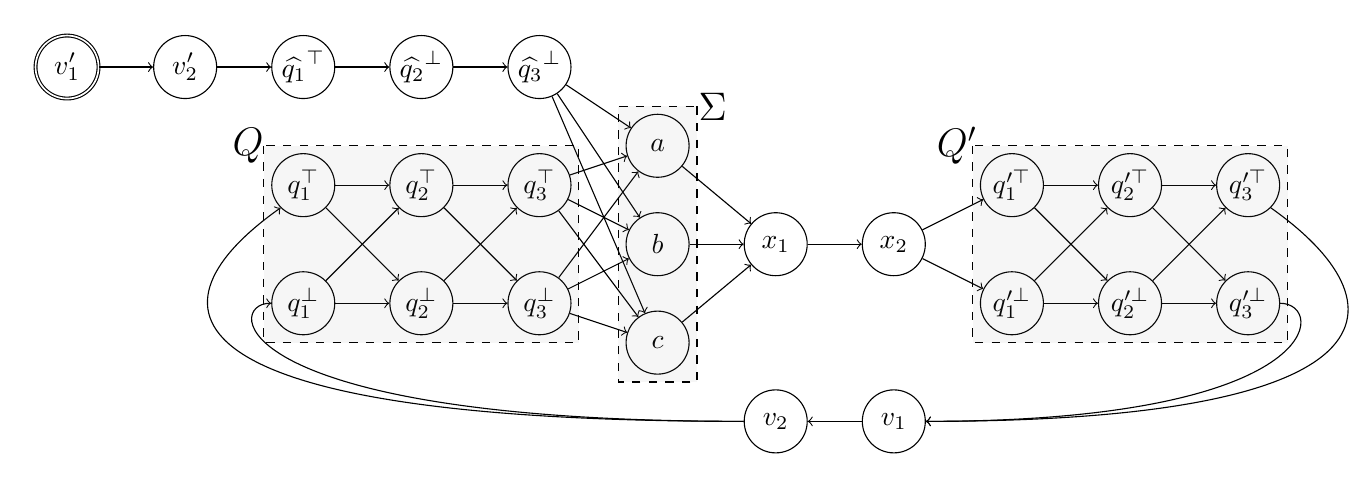
\begin{tikzpicture}[every node/.style={draw,circle,inner sep=1pt,minimum size=0.8cm}]

\draw[draw=none, use as bounding box]  (-7,5.5) rectangle (9.7,0);

\node (v1) at (-3.5,3.5) {$q_1^\top$};
\node (v4) at (-3.5,2) {$q_1^\bot$};
\node (v2) at (-2,3.5) {$q_2^\top$};
\node (v5) at (-2,2) {$q_2^\bot$};
\node (v3) at (-0.5,3.5) {$q_3^\top$};
\node (v6) at (-0.5,2) {$q_3^\bot$};
\node (v8) at (1,2.75) {$b$};
\node (v7) at (1,4) {$a$};
\node (v9) at (1,1.5) {$c$};
\node (v10) at (2.5,2.75) {$x_1$};
\node (v11) at (4,2.75) {$x_2$};
\node (v12) at (5.5,3.5) {$q_1'^\top$};
\node (v13) at (5.5,2) {$q_1'^\bot$};
\node (v16) at (7,2) {$q_2'^\bot$};
\node (v14) at (7,3.5) {$q_2'^\top$};
\node (v15) at (8.5,3.5) {$q_3'^\top$};
\node (v17) at (8.5,2) {$q_3'^\bot$};
\node (v23) at (4,0.5) {$v_1$};
\node (v24) at (2.5,0.5) {$v_2$};


\draw [->] (v1) edge (v2);
\draw [->] (v2) edge (v3);
\draw [->] (v4) edge (v5);
\draw [->] (v5) edge (v6);
\draw [->] (v4) edge (v2);
\draw [->] (v1) edge (v5);
\draw [->] (v5) edge (v3);
\draw [->] (v2) edge (v6);
\draw [->] (v3) edge (v7);
\draw [->] (v3) edge (v8);
\draw [->] (v3) edge (v9);
\draw [->] (v6) edge (v7);

\draw [->] (v6) edge (v8);
\draw [->] (v6) edge (v9);
\draw [->] (v7) edge (v10);
\draw [->] (v8) edge (v10);
\draw [->] (v9) edge (v10);
\draw [->] (v10) edge (v11);
\draw [->] (v11) edge (v12);
\draw [->] (v11) edge (v13);
\draw [->] (v12) edge (v14);
\draw [->] (v14) edge (v15);
\draw [->] (v13) edge (v16);
\draw [->] (v16) edge (v17);
\draw [->] (v13) edge (v14);
\draw [->] (v12) edge (v16);
\draw [->] (v14) edge (v17);
\draw [->] (v16) edge (v15);

\node (v22) at (-0.5,5) {$\widehat{q_3}^\bot$};
\node (v21) at (-2,5) {$\widehat{q_2}^\bot$};
\node (v20) at (-3.5,5) {$\widehat{q_1}^\top$};
\node (v19) at (-5,5) {$v_2'$};
\node [double] (v18) at (-6.5,5) {$v_1'$};
\draw [->] (v18) edge (v19);
\draw [->] (v19) edge (v20);
\draw [->] (v20) edge (v21);
\draw [->] (v21) edge (v22);
\draw [->] (v22) edge (v7);
\draw [->] (v22) edge (v8);
\draw [->] (v22) edge (v9);

\draw [->](v15.south east) .. controls (10.5,2) and (10.5,0.5) .. (v23.east);
\draw [->](v17.east) .. controls (9.5,2) and (9.5,0.5) .. (v23.east);
\draw [->] (v23) edge (v24);
\draw [->](v24.west) .. controls (-5.5,0.5) and (-5.5,2) .. (v1.south west);
\draw [->](v24.west) .. controls (-4.5,0.5) and (-4.5,2) .. (v4.west);

\draw [dashed,fill=gray,fill opacity=0.07] (-4,4) rectangle (0,1.5);
\draw [dashed,fill=gray,fill opacity=0.07]  (5,4) rectangle (9,1.5);
\draw [dashed,fill=gray,fill opacity=0.07]  (1.5,4.5) rectangle (0.5,1);

\node [draw=none] at (-4.2,4) {\Large $Q$};
\node [draw=none] at (1.7,4.5) {\Large $\Sigma$};
\node [draw=none] at (4.8,4) {\Large $Q'$};

\end{tikzpicture}}
    %\vspace*{-0.7cm}
    \caption{The Kripke structure $\Ku_\Au$ built for an $\NFA$ with set of states $Q=\{q_1,q_2,q_3\}$  and alphabet $\Sigma=\{a,b,c\}$}
    \label{fig:HardKu}
\end{sidewaysfigure}

The idea is that the computation of $\Du$ on a word, say $aab$, which we have already seen in (\ref{eq:1}), should be represented by the following initial trace of $\Ku_\Au$:
\begin{equation}\begin{split}
v_1'v_2'\underbrace{(\widehat{q_1}^\top\widehat{q_2}^\bot\widehat{q_3}^\bot)}_{Q_1} a x_1x_2 \underbrace{({q'_1}^\top {q'_2}^\top {q'_3}^\bot)}_{Q'_2}\cdots\\
v_1v_2 \underbrace{({q_1}^\top {q_2}^\top {q_3}^\bot)}_{Q_2} a x_1x_2 \underbrace{({q'_1}^\top {q'_2}^\top {q'_3}^\top)}_{Q'_3} \cdots\\
v_1v_2 \underbrace{({q_1}^\top {q_2}^\top {q_3}^\top)}_{Q_3} b x_1x_2 \underbrace{({q'_1}^\top {q'_2}^\bot {q'_3}^\top)}_{Q'_4} \cdots\\
v_1v_2 \underbrace{({q_1}^\top {q_2}^\bot {q_3}^\top)}_{Q_4}.
\end{split}
\label{eq:extrack}
\end{equation}
 
The states $v_1,v'_1,v_2,v'_2,x_1,x_2$ are there only for technical reasons (explained later). 
A triple of states $({q_1}^* {q_2}^* {q_3}^*)$ denoted by $Q_i$, where $^*$ stands for $\top$ or $\bot$,  represents a state of $\Du$, reached at the $(i-1)$-th step of the computation before reading $w(i-1)$: we have ${q_j}^\top$ if $q_j\in Q_i$, and ${q_j}^\bot$ if $q_j\not\in Q_i$.
Moreover the subtraces denoted by $Q_i$ and $Q'_i$ must be copies (i.e., ${q_j}^\top\in Q_i$ iff ${q'_j}^\top\in Q'_i$).
In between $Q_i$ and $Q'_{i+1}$ in the trace we have $w(i-1)\in\Sigma$.
The states $\widehat{q_1}^\top$, $\widehat{q_2}^\bot$ and $\widehat{q_3}^\bot$ of $\Ku_\Au$ are just \lq\lq copies\rq\rq{} of ${q_1}^\top$, ${q_2}^\bot$ and ${q_3}^\bot$ respectively, added to ensure that the first state of the $\DFA$ $\Du$ is $Q_1=\{q_1\}$ (represented by $\widehat{q_1}^\top \widehat{q_2}^\bot \widehat{q_3}^\bot$). 
Finally note that there is an intuitive match between subtraces and proposition letters satisfied. For example,
\begin{multline*}
    \Ku_\Au, v_1v_2 ({q_1}^\top {q_2}^\top {q_3}^\top) b x_1x_2 ({q'_1}^\top {q'_2}^\bot {q'_3}^\top)\models\\
    (q_1\wedge q_2\wedge q_3)\wedge (q'_1\wedge\neg q'_2\wedge q'_3)\wedge (\neg a \wedge b \wedge \neg c).
\end{multline*}

Let us now come to the formula $\Phi_\Au$, built from $\Au$. We assume the \emph{strict} semantic variant of $\hsDhom${}.
Preliminarily, we define the following formulas, which exploit the auxiliary states $v_1,v'_1,v_2,v'_2,x_1,x_2$ in order to ``select'' some suitable traces:
\[
    \varphi_{trans}=\neg f_1\wedge \neg f_2 \wedge \hsDu(f_1\wedge f_2) \wedge \hsD\top ,
\]
\[
    \varphi_{copy}= \neg e_2\wedge \neg e_1 \wedge \hsDu(e_1\wedge e_2) \wedge \hsD\top .
\]
% \[
%     \varphi'_{trans}=\neg e_2\wedge e_1 \wedge \neg f_1\wedge \neg f_2 ,
% \]
%
We can prove that:
\begin{itemize}
    \item $\Ku_\Au,\rho\models\varphi_{trans}$ if and only if $\rho=\tilde{v_2}\cdots v_1$ and $v_1,v_2$ do not occur as internal states of $\rho$ (where $\tilde{v_2}$ can be either $v_2$ or $v'_2$);
%    \item \textbf{$\Ku_\Au,\rho\models\varphi'_{trans}$ iff ($\rho=x_2\cdots v_1 v_2 q_1^*\cdots q_j^*$ for $j\geq 0$, or $\rho=x_2\cdots v_1 v_2 q_1^*\cdots q_{|Q|}^*c$ for some $c\in\Sigma$) and there are no occurrences of $x_1$ in $\rho$;}
    \item $\Ku_\Au,\rho\models\varphi_{copy}$ if and only if $\rho=x_2\cdots x_1$ and $x_1,x_2$ do not occur as internal states of $\rho$.
\end{itemize}


Moreover the following formulas have an intuitive meaning (in particular $\Length_{\geq 3}$ is satisfied by a trace $\rho$ if and only if $|\rho|\geq 3$):
\[
    \varphi_{reject}= \bigwedge_{q_i\in F}\neg q_i,
\]
% \[
%     length_{\leq|Q|+2}=\underbrace{\bD\cdots\bD}_{\lceil\frac{|Q|}{2}\rceil+1\text{ times}} \bot ,
% \]
\[
    \Length_{\geq 3}=\hsD\top .
\]

The formula $\Phi_\Au$ is defined as follows (for the sake of brevity, for $q_i,q_j\in Q$ and $c\in\Sigma$, we denote $q_j\in\Delta(q_i,c)$ as $(q_i,c,q_j)\in\Delta$).
\begin{multline*}
    \Phi_\Au=
     \underbrace{\hsDu\Big(\varphi_{trans}\rightarrow \Big(\big(\smashoperator{\bigwedge_{(q_i,a,q'_j)\in\Delta}}((q_i\wedge a)\rightarrow q'_j)\big) \wedge \big(\smashoperator{\bigwedge_{q'_i\in Q}} (q'_i\rightarrow \smashoperator{\bigvee_{(q_j,a,q'_i)\in\Delta}} (q_j\wedge a))\big) \Big)\Big)}_{(1)}\wedge\\
     \underbrace{\hsDu\big( \varphi_{copy} \rightarrow\!\! \smashoperator{\bigwedge_{q_i\in Q}} (q_i\leftrightarrow q'_i) \big)}_{(2)}\!\wedge\! \underbrace{\Big((e_1\!\wedge\! \Length_{\geq 3}\wedge \varphi_{reject})\!\vee\! \hsD\!\Big(\varphi_{copy}\!\wedge\!\varphi_{reject}\Big)\Big)}_{(3)}
\end{multline*}

%For the sake of simplicity, in the following we assume w.l.o.g.\ that $\Au$ has an even number of states (we may always add a non-final disconnected fresh state).
Let us now prove the following lemma.
\begin{lemma}\label{lemma:nuniv}
$\Lang(\Au)\neq \Sigma^*$ if and only if there exists an initial trace $\rho$ of $\Ku_\Au$ such that $\Ku_\Au,\rho\models \Phi_\Au$.
\end{lemma}
%
\begin{proof}
$(\Rightarrow)$ If $\Lang(\Au)\neq \Sigma^*$, then there is $w\notin\Lang(\Au)$. Therefore the computation of $\Du$ over $w$ is \emph{not} accepting. Let us consider the initial trace $\rho$ of $\Ku_\Au$ encoding such a computation as explained before, see (\ref{eq:extrack}). We distinguish two cases:
\begin{itemize}
    \item $w=\varepsilon$: then we consider $\rho=v'_1v'_2\widehat{q_1}^\top\widehat{q_2}^\bot\cdots \widehat{q_{|Q|}}^\bot $. No strict subtrace satisfies $\varphi_{trans}$ or $\varphi_{copy}$, hence conjuncts (1) and (2) are trivially satisfied. Moreover, since $\varepsilon\notin\Lang(\Au)$, $q_1\notin F$, thus $\rho$ models also $e_1\wedge \Length_{\geq 3}\wedge \varphi_{reject}$.
    \item $w\neq \varepsilon$; then we consider the initial trace $\rho$ of $\Ku_\Au$ encoding the computation over $w$, w.l.o.g.\ extended with some $c\in\Sigma$ (any symbol is fine), and finally $x_1x_2$: its generic form is $\rho=v'_1v'_2\widehat{q_1}^\top\widehat{q_2}^\bot\cdots \widehat{q_{|Q|}}^\bot w(0)(x_1x_2{q'_1}^*{q'_2}^*\cdots {q'_{|Q|}}^*\cdot\allowbreak v_1v_2{q_1}^*{q_2}^*\cdots {q_{|Q|}}^*c)^+x_1x_2$, where $^*$ is $^\bot$ or $^\top$, and $^+$ denotes a positive number of occurrences of the string in brackets. Every strict subtrace satisfying $\varphi_{trans}$ models the right part of the implication in conjunct (1), which enforces the consistency conditions of a computation. 
    Every strict subtrace satisfying $\varphi_{copy}$ features ${q'_i}^\top$ if it features ${q_i}^\top$, and ${q'_i}^\bot$ if it features ${q_i}^\bot$, hence it satisfies $\bigwedge_{q_i\in Q} (q_i\leftrightarrow q'_i)$. Finally, the last part of $\rho$, $x_2{q'_1}^*{q'_2}^*\cdots {q'_{|Q|}}^*v_1v_2{q_1}^*{q_2}^*\cdots {q_{|Q|}}^*c x_1$,
    models $\varphi_{copy}$, and, since $w$ is \emph{not} accepted, it also fulfills $\varphi_{reject}$.
\end{itemize}
Therefore, in both cases, there exists an initial trace $\rho$ such that $\Ku_\Au,\rho\models \Phi_\Au$.

$(\Leftarrow)$ Let us assume there exists an initial trace $\rho$ of $\Ku_\Au$ such that $\Ku_\Au,\rho\models \Phi_\Au$. We distinguish some cases, according to the structure of $\rho$.
\begin{enumerate}
    \item $\rho=v'_1(v'_2)^?$ ($^?$ denotes 0 or 1 occurrences of the string in brackets).\\ 
    This trace does not model (3), thus it cannot be the trace we are looking for.
    %
    \item $\rho\!=\!v'_1v'_2\widehat{q_1}^\top\widehat{q_2}^\bot \cdots \widehat{q_j}^\bot$ for $j\geq 1$, or $\rho\!=\!v'_1v'_2\widehat{q_1}^\top\widehat{q_2}^\bot \cdots \widehat{q_{|Q|}}^\bot c$ for some $c\!\in\!\Sigma$.\\
    No subtrace satisfies $\varphi_{copy}$, thus, by the conjunct (3), $\rho$ models $\varphi_{reject}$. Hence $q_1\notin F$, and $\varepsilon$ is rejected by $\Au$.
    %
    \item $\rho=v'_1v'_2\widehat{q_1}^\top\widehat{q_2}^\bot \cdots \widehat{q_{|Q|}}^\bot c x_1(x_2)^?$\\
    This trace does not model the conjunct (3).
    %
    \item $\rho=v'_1v'_2\widehat{q_1}^\top\widehat{q_2}^\bot \cdots \widehat{q_{|Q|}}^\bot c x_1x_2{q'_1}^*{q'_2}^*\cdots {q'_j}^*$  for $j\geq 1$\\
    This trace does not model the conjunct (3).
    %
    \item $\rho=v'_1v'_2\widehat{q_1}^\top\widehat{q_2}^\bot \cdots \widehat{q_{|Q|}}^\bot c x_1x_2{q'_1}^*{q'_2}^*\cdots {q'_{|Q|}}^*v_1(v_2)^?$\\
    This trace does not model the conjunct (3).
    %
    \item $\rho=v'_1v'_2\widehat{q_1}^\top\widehat{q_2}^\bot \cdots \widehat{q_{|Q|}}^\bot c x_1x_2{q'_1}^*{q'_2}^*\cdots {q'_{|Q|}}^*v_1v_2{q_1}^*{q_2}^*\cdots {q_j}^*$\\
    This trace does not model the conjunct (3).
    %
    \item $\rho=v'_1v'_2\widehat{q_1}^\top\widehat{q_2}^\bot \cdots \widehat{q_{|Q|}}^\bot c x_1x_2{q'_1}^*{q'_2}^*\cdots {q'_{|Q|}}^*v_1v_2{q_1}^*{q_2}^*\cdots {q_{|Q|}}^*c$\\
    This trace does not model the conjunct (3).
    %
    \item $\rho=v'_1v'_2\widehat{q_1}^\top\widehat{q_2}^\bot \cdots \widehat{q_{|Q|}}^\bot c x_1x_2{q'_1}^*{q'_2}^*\cdots {q'_{|Q|}}^*v_1v_2{q_1}^*{q_2}^*\cdots {q_{|Q|}}^*cx_1$\\
    This trace does not model the conjunct (3).
    %
    \item\label{case:A} $\rho=v'_1v'_2\widehat{q_1}^\top\widehat{q_2}^\bot \cdots \widehat{q_{|Q|}}^\bot c (x_1x_2{q'_1}^*{q'_2}^*\cdots {q'_{|Q|}}^*v_1v_2{q_1}^*{q_2}^*\cdots {q_{|Q|}}^*c)^+x_1x_2$\\
    We have that, since $\rho$ models the conjunct (1), \emph{all} adjacent pairs of occurrences of ${q_1}^*{q_2}^*\cdots {q_{|Q|}}^*\rightsquigarrow{q'_1}^*{q'_2}^*\cdots {q'_{|Q|}}^*$ consistently model a transition of $\Du$; moreover \emph{all} adjacent pairs of occurrences of ${q'_1}^*{q'_2}^*\cdots {q'_{|Q|}}^*\rightsquigarrow {q_1}^*{q_2}^*\cdots {q_{|Q|}}^*$ are ``copies''. Put all together, a legal computation of $\Du$ over some string $w$ is encoded. 
    Finally, by the conjunct (3), a strict subtrace $x_2{q'_1}^*{q'_2}^*\cdots {q'_{|Q|}}^*v_1v_2{q_1}^*{q_2}^*\cdots {q_{|Q|}}^*c x_1$ models $\varphi_{reject}$. Thus either $w$ (if such subtrace is the last one) or one of its prefixes (if it is not the last one) is rejected by $\Du$.
    %
    \item\label{case:B} $\rho=v'_1v'_2\widehat{q_1}^\top\widehat{q_2}^\bot \cdots \widehat{q_{|Q|}}^\bot c (x_1x_2{q'_1}^*{q'_2}^*\cdots {q'_{|Q|}}^*v_1v_2{q_1}^*{q_2}^*\cdots {q_{|Q|}}^*c)^+x_1x_2\cdot\allowbreak \underline{{q'_1}^*{q'_2}^*\cdots {q'_j}^*}$\\
    In this case and in the following ones, we underline the final part of $\rho$ which may be ``garbage'', namely, it may encode an illegal suffix of a computation, just because it is not forced to ``behave correctly'' by $\Phi_\Au$.
    However, since conjunct (3) is satisfied, a strict subtrace $x_2{q'_1}^*{q'_2}^*\!\cdots {q'_{|Q|}}^*v_1v_2{q_1}^*{q_2}^*\!\cdots {q_{|Q|}}^*c x_1$ models $\varphi_{reject}$ (and this is not part of the garbage). Thus, as before, some word $w$ or one of its prefixes is rejected by $\Du$.
    %
    \item $\rho=v'_1v'_2\widehat{q_1}^\top\widehat{q_2}^\bot \cdots \widehat{q_{|Q|}}^\bot c (x_1x_2{q'_1}^*{q'_2}^*\cdots {q'_{|Q|}}^*v_1v_2{q_1}^*{q_2}^*\cdots {q_{|Q|}}^*c)^+x_1x_2\cdot\allowbreak\underline{{q'_1}^*{q'_2}^*\cdots {q'_{|Q|}}^*v_1}$\\
    Like the previous case.
    %
    \item\label{case:C} 
    $
    \rho=v'_1v'_2\widehat{q_1}^\top\widehat{q_2}^\bot \cdots \widehat{q_{|Q|}}^\bot c (x_1x_2{q'_1}^*{q'_2}^*\cdots {q'_{|Q|}}^*v_1v_2{q_1}^*{q_2}^*\cdots {q_{|Q|}}^*c)^+x_1x_2\cdot \allowbreak
    {q'_1}^*{q'_2}^*\cdots {q'_{|Q|}}^*v_1v_2
    $\\
    Like case~\ref{case:A}, but a prefix of $w$ is necessarily rejected, such that $\rho$ encodes the computation of $\Du$ over $w$.
    %
    \item 
        $
        \rho=v'_1v'_2\widehat{q_1}^\top\widehat{q_2}^\bot \cdots \widehat{q_{|Q|}}^\bot c (x_1x_2{q'_1}^*{q'_2}^*\cdots {q'_{|Q|}}^*v_1v_2{q_1}^*{q_2}^*\cdots {q_{|Q|}}^*c)^+x_1x_2\cdot \allowbreak 
        {q'_1}^*{q'_2}^*\cdots {q'_{|Q|}}^*v_1v_2\underline{{q_1}^*{q_2}^*\cdots {q_j}^*},
        $
        \\
        $
        \rho=v'_1v'_2\widehat{q_1}^\top\widehat{q_2}^\bot \cdots \widehat{q_{|Q|}}^\bot c (x_1x_2{q'_1}^*{q'_2}^*\cdots {q'_{|Q|}}^*v_1v_2{q_1}^*{q_2}^*\cdots {q_{|Q|}}^*c)^+x_1x_2\cdot \allowbreak
        {q'_1}^*{q'_2}^*\cdots {q'_{|Q|}}^*v_1v_2\underline{{q_1}^*{q_2}^*\cdots {q_{|Q|}}^*c},
        $
        \\
        $
        \rho=v'_1v'_2\widehat{q_1}^\top\widehat{q_2}^\bot \cdots \widehat{q_{|Q|}}^\bot c (x_1x_2{q'_1}^*{q'_2}^*\cdots {q'_{|Q|}}^*v_1v_2{q_1}^*{q_2}^*\cdots {q_{|Q|}}^*c)^+x_1x_2\cdot \allowbreak
        {q'_1}^*{q'_2}^*\cdots {q'_{|Q|}}^*v_1v_2\underline{{q_1}^*{q_2}^*\cdots {q_{|Q|}}^*c x_1}.
        $ 
    
   All like case~\ref{case:C}, just with the addition of final garbage, which is not considered, since it is not part of a strict subtrace satisfying $\varphi_{copy}$.
\end{enumerate}
Thus, in all possible (legal) cases, some string is rejected by $\Du$ (and by $\Au$).
\end{proof}

It follows that $\Lang(\Au)= \Sigma^*$ if and only if $\Ku_\Au\models \neg\Phi_\Au$. Since also the \emph{problem of universality} of the language of an $\NFA$ is $\Psp$-complete (because $\Psp$ is closed under complement), and both $\Ku_\Au$ and $\Phi_\Au$ can be generated in polynomial time, 
we have proved the following.
\begin{theorem}
The MC problem for $\hsDhom$ formulas over finite Kripke structures is $\Psp$-hard (under polynomial-time reductions).
\end{theorem}
%
By slightly modifying $\Phi_\Au$, we can adapt the proof to the \emph{proper} variant of $\hsDhom${}.


\section{$\Psp$-Hardness of SAT for $\hsDhom${} over finite linear orders}\label{sec:SAThard}
In this section we outline a $\Psp$-hardness proof for the SAT problem 
for $\hsDhom$ formulas over finite linear orders.

The construction mimics that of Sections 3.2 and 3.3 of \cite{DBLP:journals/fuin/MarcinkowskiM14}, in which the authors show 
that it is possible to build a formula $\Psi$ of $\D$ which encodes accepting computations of an $\NFA$. More precisely the set of letters of $\Psi$ equals the union of the alphabet of the $\NFA$ and the set of its states (plus some auxiliary letters, to enforce the \lq\lq orientation\rq\rq{} in the linear order, something that $\D${} is unaware of), and $\Psi$ is satisfied by all and only the models such that the point-intervals are labeled with an accepting computation of the $\NFA$ over the word written in its point-intervals.

The idea is then to exploit $\Psi$ to encode the Kripke structure of the previous section, thus getting a reduction from the 
problem of non-universality of the language of an $\NFA$ to the SAT problem for $\hsDhom$.
As a matter of fact, a Kripke structure can be regarded as a trivial $\NFA$ over a unary alphabet, say $\{a\}$, such that all the states are final, as we are interested only in the structure of traces (i.e., any word/trace is accepted under the only constraint that it exists in the structure).

By an easy adaptation of the results of Sections 3.2 and 3.3 of \cite{DBLP:journals/fuin/MarcinkowskiM14} we get the following.
\begin{proposition}\label{prop:MM}
    Given a Kripke structure $\Ku=\KuDef$ devoid of self-loops, there exists a $\hsDhom$ formula $\Psi_{\Ku}$ whose set of proposition letters is $\AP\cup\States\cup Aux$---being $Aux$ a set of auxiliary letters---such that any finite linear order satisfying $\Psi_{\Ku}$ represents an initial trace of $\Ku$.
    Moreover $\Psi_{\Ku}$ is polynomial in the size of $\Ku$.
\end{proposition}
Every linear order satisfying $\Psi_{\Ku}$ features states of $\Ku$ labeling point-intervals (exactly one state for each point). 
Moreover we can easily force, for each occurrence of some state $s$ of $\Ku$ along the order, the set of letters $\Lab(s)$ to hold on the same position (point).
The structure $\Ku$ in Proposition~\ref{prop:MM} must not feature self-loops for a technical reason: by fulfilling this requirement, there is no way for a state of $\Ku$ to \lq\lq span\rq\rq{} (by homogeneity) more than one point in a linear order satisfying $\Psi_{\Ku}$. 
%
We observe that in~\cite{DBLP:journals/fuin/MarcinkowskiM14} the authors do not assume homogeneity; however homogeneity does not cause problems in our construction, as, intuitively, all the significant properties stated by $\Psi_{\Ku}$ are related to point-intervals. 

Let us observe that the Kripke structure of the previous section does not contain self-loops.
%
By Lemma~\ref{lemma:nuniv}, the language of an $\NFA$ $\Au$ is non-universal if and only if there exists an initial trace $\rho$ such that $\Ku_\Au,\rho\models \Phi_\Au$ (the Kripke structure and formula built from $\Au$ in the previous section), if and only if (by Proposition~\ref{prop:MM} applied to $\Ku_\Au$) the formula $\Psi_{\Ku_\Au}\wedge\Phi_\Au$ is satisfiable. We have proved the following result.
%
\begin{theorem}
The SAT problem for $\hsDhom$ formulas over finite linear orders is $\Psp$-hard.
\end{theorem}